%
% svdmotivation.tex
%
% (c) 2018 Prof Dr Andreas Müller, Hochschule Rapperswil
%
\documentclass[tikz,12pt]{standalone}
\usepackage{times}
\usepackage{amsmath}
\usepackage{txfonts}
\usepackage[utf8]{inputenc}
\usepackage{graphics}
\usepackage{color}
\usepackage{pifont}
\usetikzlibrary{arrows,intersections,math,calc}
\begin{document}

\def\punkt#1{
        \fill[color=white] #1 circle[radius=0.08];
        \draw #1 circle[radius=0.08];
}

\begin{tikzpicture}[>=latex,thick]

\begin{scope}[xshift=-4cm]
\node at (0,0) {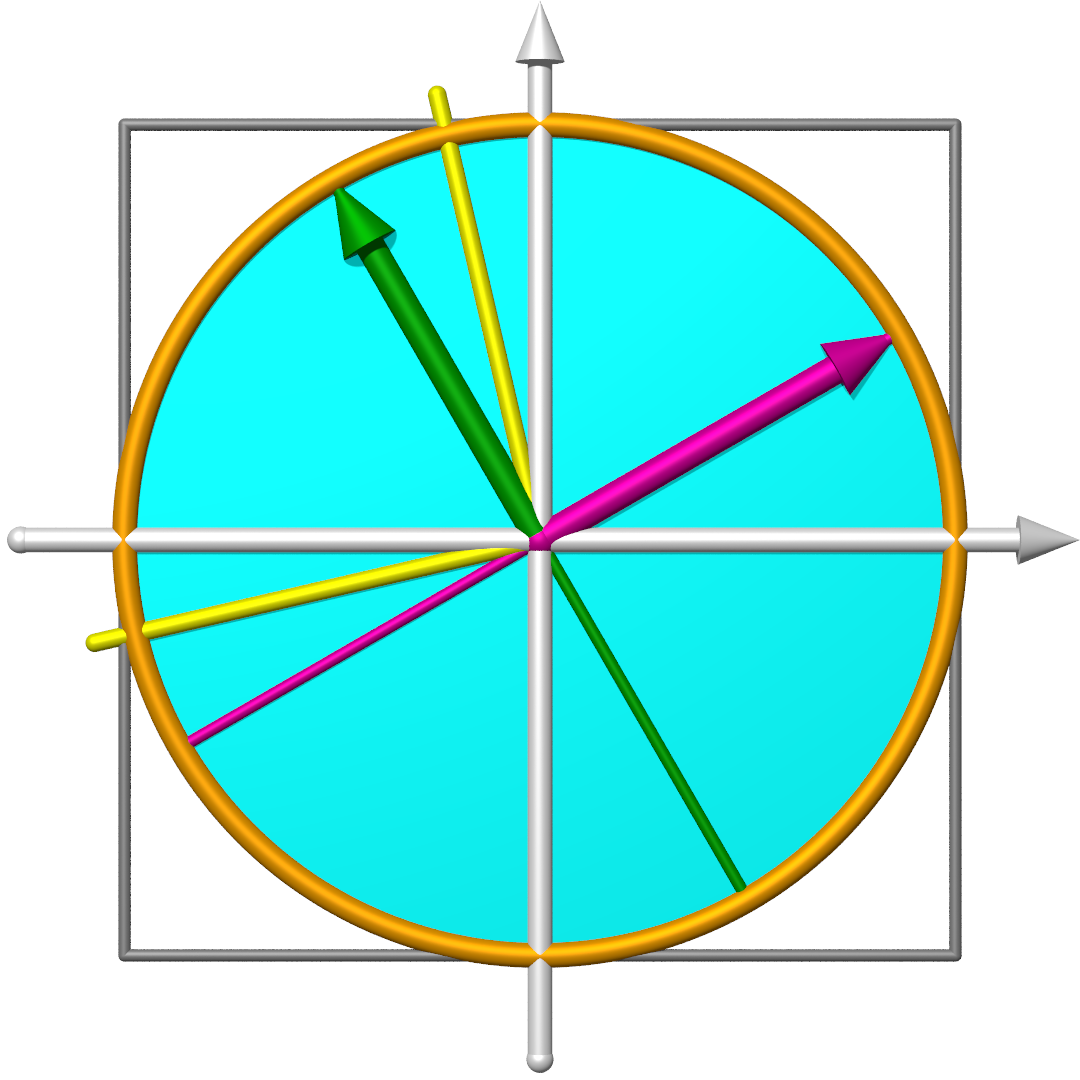
\includegraphics[width=4cm]{circle-coord.png}};
\node at (0.82,0.88) {$\vec{v}_1$};
\node at (-0.7,0.7) {$\vec{v}_2$};
\end{scope}

\begin{scope}[xshift=5cm]
\node at (0,0) {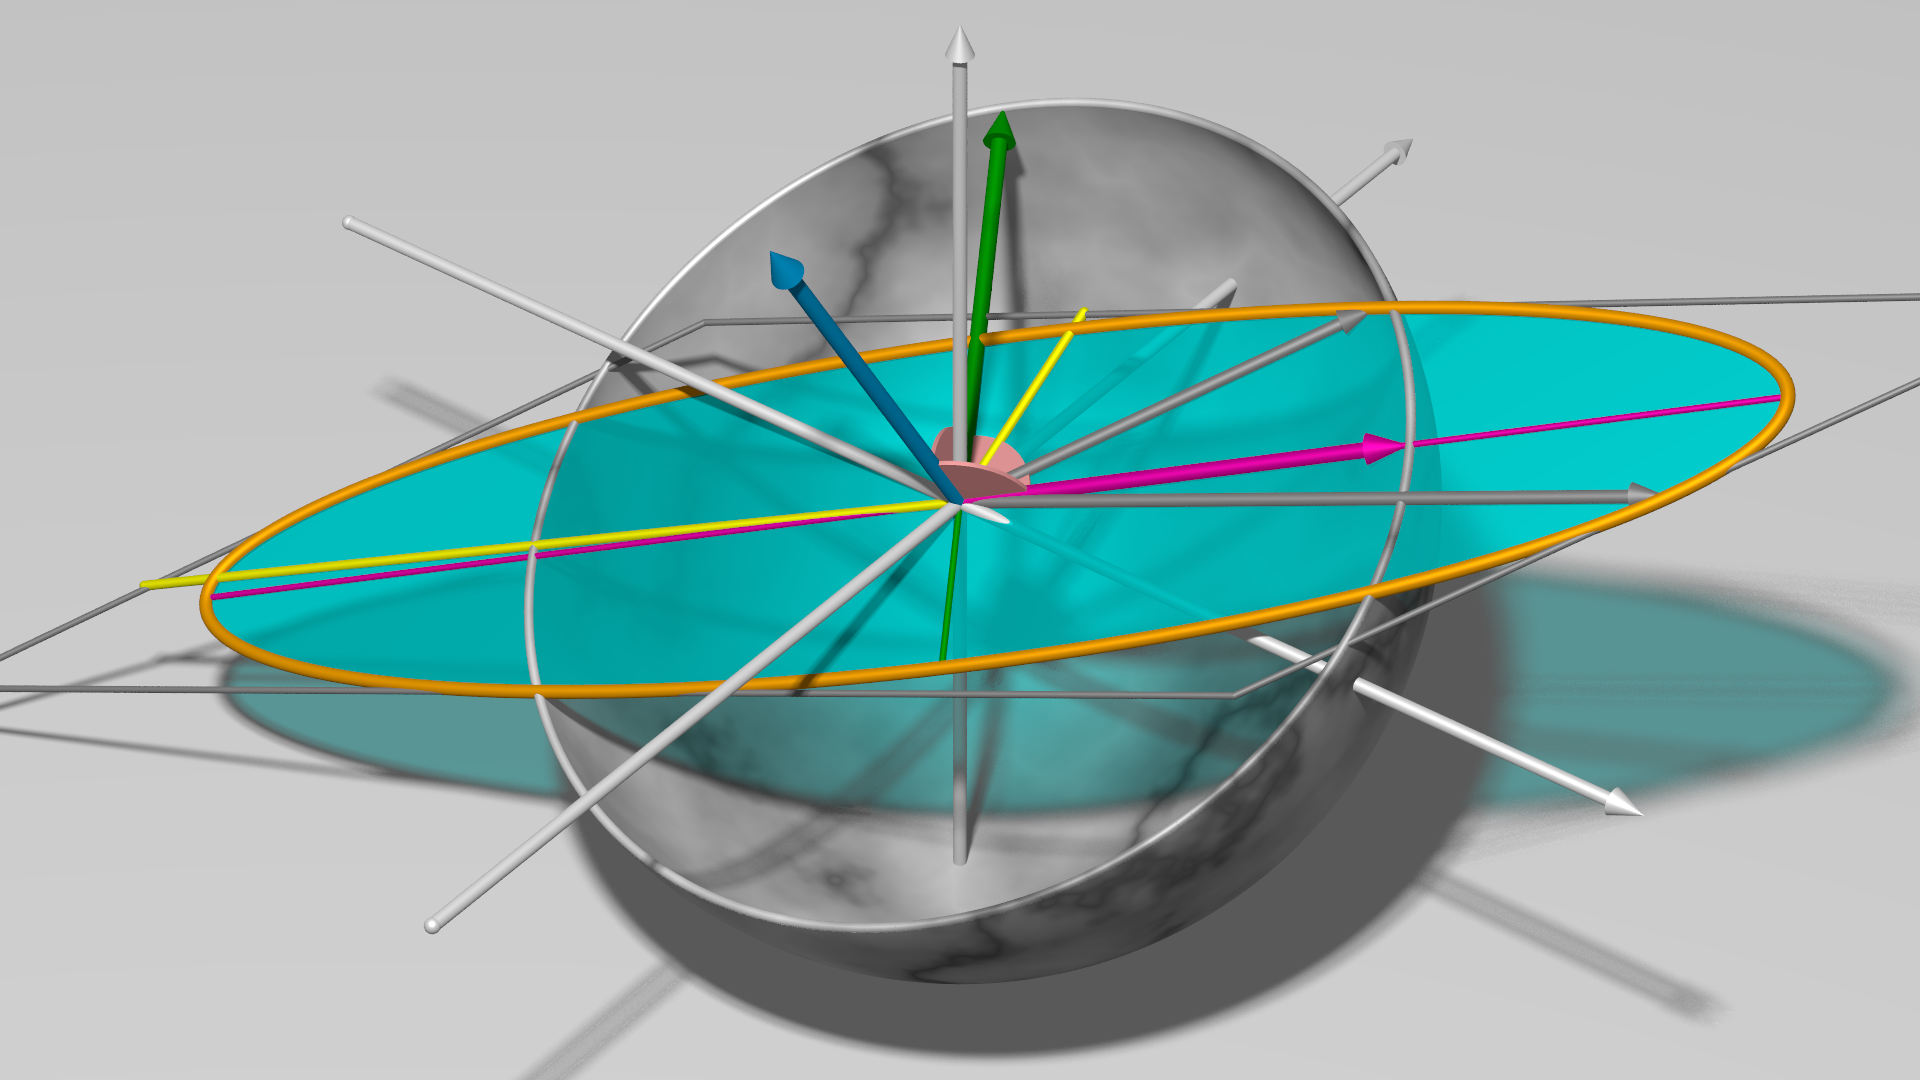
\includegraphics[width=10cm]{ellipse-coord.png}};
\node at (2.3,0.8) {$\vec{u}_1$};
\node at (0.3,2.5) {$\vec{u}_2$};
\node at (-1.2,1.4) {$\vec{u}_3$};
\end{scope}

\begin{scope}[xshift=-1.2cm,yshift=-2.9cm]
\node at (0,3.3) [above] {$A$};
\draw[<-] (70:3.3) arc (70:110:3.3);
\end{scope}

\end{tikzpicture}

\end{document}

